\chapter{C Programming for Beginners} \label{chp:chapter_cl}

    Welcome to the \autoref{chp:chapter_cl}, dedicated to the fundamentals of the C language. As an instructor, it is essential to acknowledge that some students may begin their journey in this discipline with limited knowledge of the C language. Understanding this, we have designed this chapter to serve as a gentle reminder and refresher on the crucial concepts that form the building blocks of the C programming.
    
    In the following sections, we will explore key aspects that every student should be familiar with to confidently navigate the world of C programming. These subsections will provide a comprehensive overview of the fundamental components necessary for developing robust and efficient code.
    
    \autoref{sec:section_cl.1}:
    In this subsection, we will delve into the significance of include statements in C programming. Understanding how to use these statements effectively allows us to incorporate external libraries and headers into our code, enabling access to additional functionalities and resources.
    
    \autoref{sec:section_cl.2}:
    Preprocessor definitions play a vital role in C programming as they provide a mechanism for modifying the source code before compilation. In this subsection, we will explore the syntax and usage of preprocessor directives, such as defining constants, macros, and conditional compilation, to enhance the flexibility and versatility of our programs.
    
    \autoref{sec:section_cl.3}:
    Variables are the cornerstone of any programming language, including C. This subsection will revisit the concept of variables, their declaration, and initialization in C. Understanding how to effectively work with variables is essential for storing, manipulating, and retrieving data during program execution.
    
    \autoref{sec:section_cl.4}:
    Operators, conditional statements, and loops form the core control structures in C programming. In this subsection, we will review the different types of operators, explore conditional statements (such as if-else and switch-case), and demonstrate how to use loops (such as for, while, and do-while) to create iterative and decision-making constructs.
    
    \autoref{sec:section_cl.5}:
    Functions provide modularity and code reusability in C programming. In this subsection, we will discuss the importance of functions, their declaration, definition, and usage. Additionally, we will explore function parameters, return types, and the concept of scope, helping students grasp the significance of functions in organizing and structuring their programs effectively.
    
    By immersing ourselves in these sections and reinforcing the fundamental concepts of C programming, both you as the instructor and your students can establish a solid foundation upon which to build further knowledge and expertise in this discipline. So let us embark on this journey and delve into the intricacies of the C language together!
    
    \section{Include Statements} \label{sec:section_cl.1}
        These statements are used to introduce the contents of a separate file into your source file. This is a handy way to keep your code organized, and it also allows you to use library functionality, hardware-configuration routines, and register definitions provided by the manufacturer.
    
            \begin{lstlisting}[style=mystyle_c, language=c, breaklines]
                /************************************************************//**
                 * Includes
                 ***************************************************************/
                #include // SFR declarations
                #include Project_DefsVarsFuncs.h
                #include InitDevice.h
                #include cslib_config.h
                #include cslib.h
            \end{lstlisting}

    \section{Preprocessor Definitions} \label{sec:section_cl.2}

        Preprocessors are programs that process the source code before compilation. A number of steps are involved between writing a program and executing a program in C / C++. Let us have a look at these steps before we actually start learning about Preprocessors.

        \begin{figure}[!ht]
                \centering
                \captionsetup{justification=centering,margin=0.05cm}
                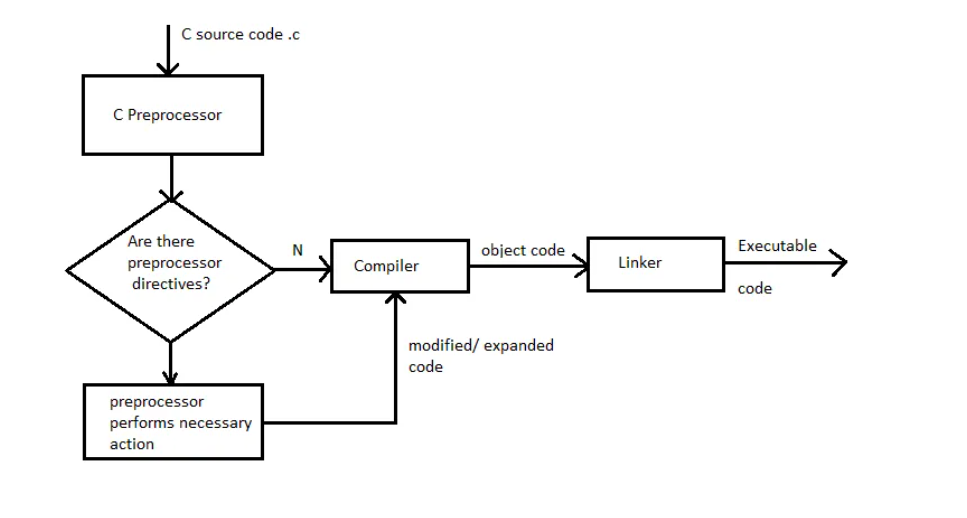
\includegraphics[width=0.8\columnwidth]{figures/preprocessor-in-c.png}
                \caption{\label{fig:preprocessor}Preprocessor in C}
        \end{figure}

        You can see the intermediate steps in the above diagram. The source code written by programmers is first stored in a file, let the name be “program.c“. This file is then processed by preprocessors and an expanded source code file is generated named “program.i”. This expanded file is compiled by the compiler and an object code file is generated named “program.obj”. Finally, the linker links this object code file to the object code of the library functions to generate the executable file “program.exe”. 

        Preprocessor programs provide preprocessor directives that tell the compiler to preprocess the source code before compiling. All of these preprocessor directives begin with a ‘\#’ (hash) symbol. The ‘\#’ symbol indicates that whatever statement starts with a ‘\#’ will go to the preprocessor program to get executed. We can place these preprocessor directives anywhere in our program.

        \begin{figure}[!ht]
                \centering
                \captionsetup{justification=centering,margin=0.05cm}
                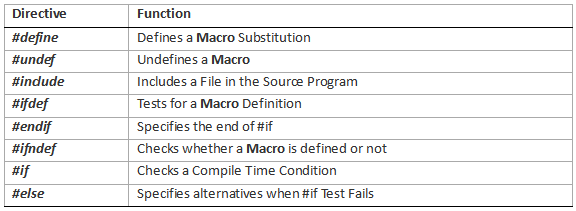
\includegraphics[width=0.8\columnwidth]{figures/preprocessor-directives.png}
                \caption{\label{fig:preprocessor-directives}All the preprocessor directives in C}
        \end{figure}

         Macros are pieces of code in a program that is given some name. Whenever this name is encountered by the compiler, the compiler replaces the name with the actual piece of code. The ‘\#define’ directive is used to define a macro. Syntax of macro definition:

         \begin{lstlisting}[style=mystyle_c, language=c, breaklines]
                #define token value
        \end{lstlisting}
    
    
        For example, let’s say that you’re using the microcontroller’s ADC and that your code uses the ADC’s sample rate in several separate calculations. A preprocessor definition allows you to use an intuitive string (such as SAMPLE\_RATE) instead of the number itself in the calculation code, and if you’re experimenting with different sample rates, you only need to change the one numerical value in the preprocessor definition.
    
            \begin{lstlisting}[style=mystyle_c, language=c, breaklines]
                #define SAMPLE_RATE 100000
            \end{lstlisting}
        
        You can change 100000 to any other number, and this new number will be used to replace all instances of the string SAMPLE\_RATE.

        Preprocessor definitions are also a great way to make code more readable. The following is a list of handy \#define statements.
     
            \begin{lstlisting}[style=mystyle_c, language=c, breaklines]
                #define BIT7 0x80
                #define BIT6 0x40
                #define BIT5 0x20
                #define BIT4 0x10
                #define BIT3 0x08
                #define BIT2 0x04
                #define BIT1 0x02 
                #define BIT0 0x01
                
                #define HIGH 1
                #define LOW 0
                
                #define TRUE 1
                #define FALSE 0
                
                #define SET 1
                #define CLEARED 0
                
                #define LOWBYTE(v)   ((unsigned char) (v))
                #define HIGHBYTE(v)  ((unsigned char) (((unsigned int) (v)) >> 8))
            \end{lstlisting}

        Its important to understand that preprocessor definitions have no direct relationship to hardware. You’re just telling the preprocessor to replace one string of characters with another string of characters before the program is compiled.
    
    \section{Variables} \label{sec:section_cl.3}
        Processors store data in registers and memory locations. There really is no such thing as a variable as far as the hardware is concerned. For the programmer, though, writing code is much easier when we can use intuitively named variables instead of memory addresses or register numbers.
            
        Compilers can manage the low-level details associated with variables without much input from the programmer, but if you want to optimize your use of variables you'll need to know something about the device’s memory configuration and the way in which it handles data of different bit widths.

        \begin{figure}[!ht]
                \centering
                \captionsetup{justification=centering,margin=0.05cm}
                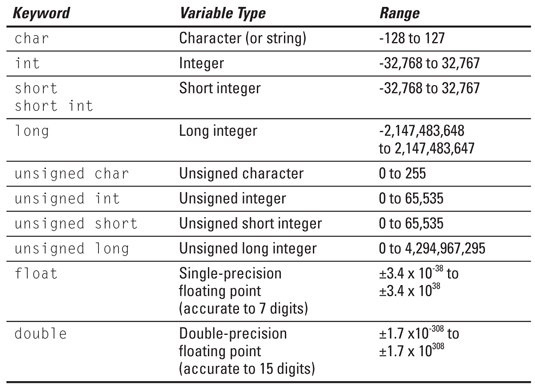
\includegraphics[width=0.8\columnwidth]{figures/variable-in-c.jpg}
                \caption{\label{fig:variable-in-c}Variable types in C}
        \end{figure}
            
        The following code excerpt gives an example of variable definition. This was written for the Keil Cx51 compiler, which reserves one byte of memory for an “unsigned char” definition, two bytes for an “unsigned int” definition, and four bytes for an “unsigned long” definition.
            
                 
            \begin{lstlisting}[style=mystyle_c, language=c, breaklines]
                unsigned long Accumulated_Capacitance_Sensor1;
                unsigned long Accumulated_Capacitance_Sensor2;
                    
                unsigned int Sensor1_Unpressed;
                unsigned int Sensor2_Unpressed;
                    
                unsigned int Sensor1_Measurement;
                unsigned int Sensor2_Measurement;
                    
                unsigned int AngularPosition;
                    
                unsigned int TouchDuration;
                    
                unsigned char CurrentDigit;
                unsigned int CharacterEntry;
                unsigned char DisplayDivider;
            \end{lstlisting}
                

    \section{Operators, Conditional Statements, and Loops} \label{sec:section_cl.4} 
        \subsection{Operators}
        
            The core of computational functionality consists of moving data, performing mathematical computations and logical operations with data, and making programmatic decisions based on the value of stored or generated data.
                
            Mathematical operations and bit manipulation are accomplished by means of operators. C has quite a few operators: equals (=), addition (+), subtraction (-), multiplication (*), division (/), bitwise AND (\&), bitwise OR (|), and so forth. The ``input'' to an operator statement are variables or constants, and the result is stored in a variable. Can you see some operators in \autoref{fig:operators-in-c}.
    
            \begin{figure}[!ht]
                    \centering
                    \captionsetup{justification=centering,margin=0.05cm}
                    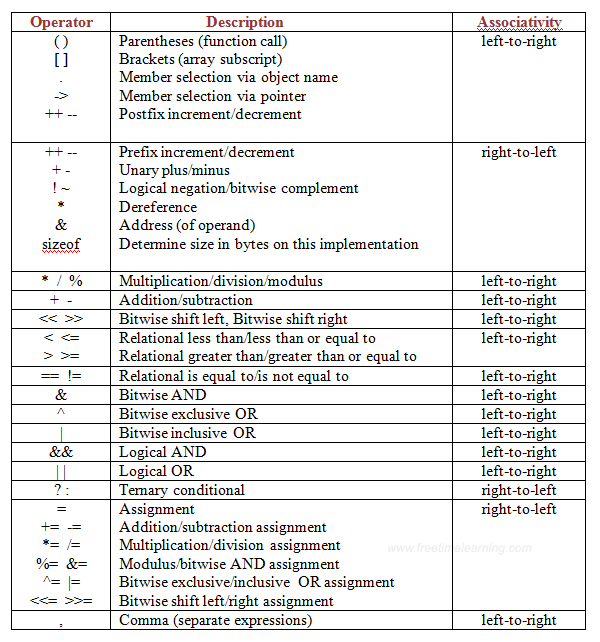
\includegraphics[width=\columnwidth]{figures/operators-in-c.png}
                    \caption{\label{fig:operators-in-c}Operators in C}
            \end{figure}

        \subsection{Conditional Statements}
            
            Conditional statements allow you to perform or not perform an action based on whether a given condition is true or false. These statements use the words \textit{“if”} and \textit{“else”}; for example:
                
                \begin{lstlisting}[style=mystyle_c, language=c, breaklines]
                    if(Sensor1 < Sensor2 && Sensor1 < Sensor3)
                        return SENSOR_1;   
                    else 
                    if(Sensor2 < Sensor1 && Sensor2 < Sensor3)
                        return SENSOR_2;     
                    else 
                    if(Sensor3 < Sensor2 && Sensor3 < Sensor1)
                        return SENSOR_3;     
                    else
                        return 0;
                \end{lstlisting} 
    
            \vspace{2cm}
            
        \subsection{Loop}
            For loops and \textit{while} loops provide a convenient means of repeatedly executing a block of code. These types of tasks arise very frequently in embedded applications. For loops are more oriented toward situations in which a block of code must be executed a specific number of times, and \textit{while} loops are handy when the processor should continue repeating the same block of code until a condition changes from true to false. The \autoref{fig:for-loop} explain the working flow of For loop and \autoref{fig:while-loop} explain the \textit{while} loop.
            
                \begin{figure}[!ht]
                    \centering
                    \captionsetup{justification=centering,margin=0.05cm}
                    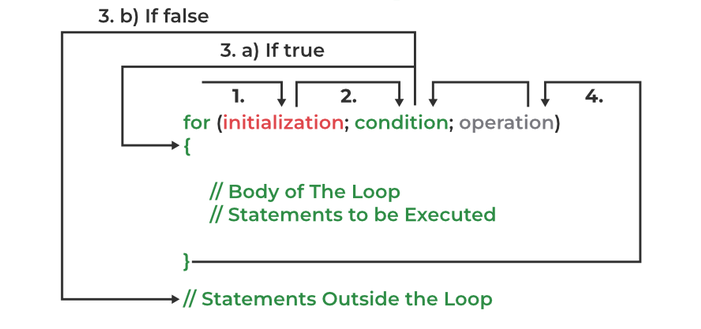
\includegraphics[width=0.8\textwidth]{figures/for-loop.png}
                    \caption{\label{fig:for-loop}For loop in C}
                \end{figure}
    
                \begin{figure}[!ht]
                    \centering
                    \captionsetup{justification=centering,margin=0.05cm}
                    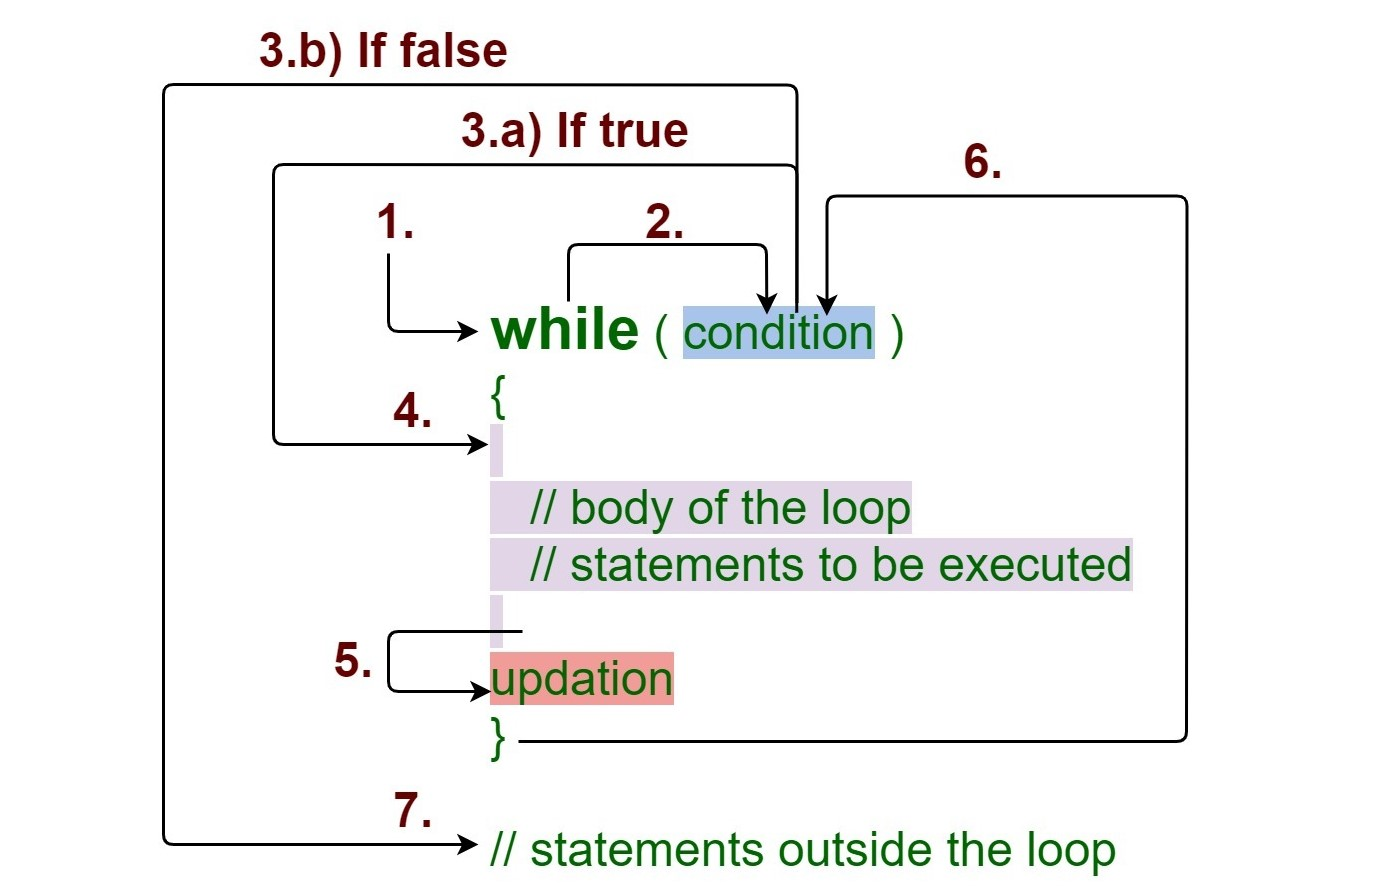
\includegraphics[width=0.7\textwidth]{figures/while-loop.jpg}
                    \caption{\label{fig:while-loop}While loop in C}
                \end{figure}
            \vspace{3cm}
                
            
            Here are examples of both types.
    
                \begin{lstlisting}[style=mystyle_c, language=c, breaklines]
                    for (n = 0; n < 16; n++)
                    {
                        Accumulated_Capacitance_Sensor1 += Measure_Capacitance(SENSOR_1);
                        Delay_us(50);
                        Accumulated_Capacitance_Sensor2 += Measure_Capacitance(SENSOR_2);
                        Delay_us(50);
                    }
                        
                    while(CONVERSION_DONE == FALSE);
                    {
                        LED_STATE = !LED_STATE;
                        Delay_ms(100);
                    }
                    \end{lstlisting}

                    
        \subsection{Switch Case}
            \textit{Switch case} statement evaluates a given expression and based on the evaluated value (matching a certain condition), it executes the statements associated with it. Basically, it is used to perform different actions based on different conditions (cases). 
        
            \begin{itemize}
                \item \textit{Switch case} statements follow a selection-control mechanism and allow a value to change control of execution.
                \item They are a substitute for long if statements that compare a variable to several integral values.
                \item They are a substitute for long if statements that compare a variable to several integral values.
                \item The switch statement is a multiway branch statement. It provides an easy way to dispatch execution to different parts of code based on the value of the expression.
            \end{itemize}
            
            In C, the \textit{switch case} statement is used for executing one condition from multiple conditions. It is similar to an if-else-if ladder.
        
            \begin{figure}[!ht]
                        \centering
                        \captionsetup{justification=centering,margin=0.05cm}
                        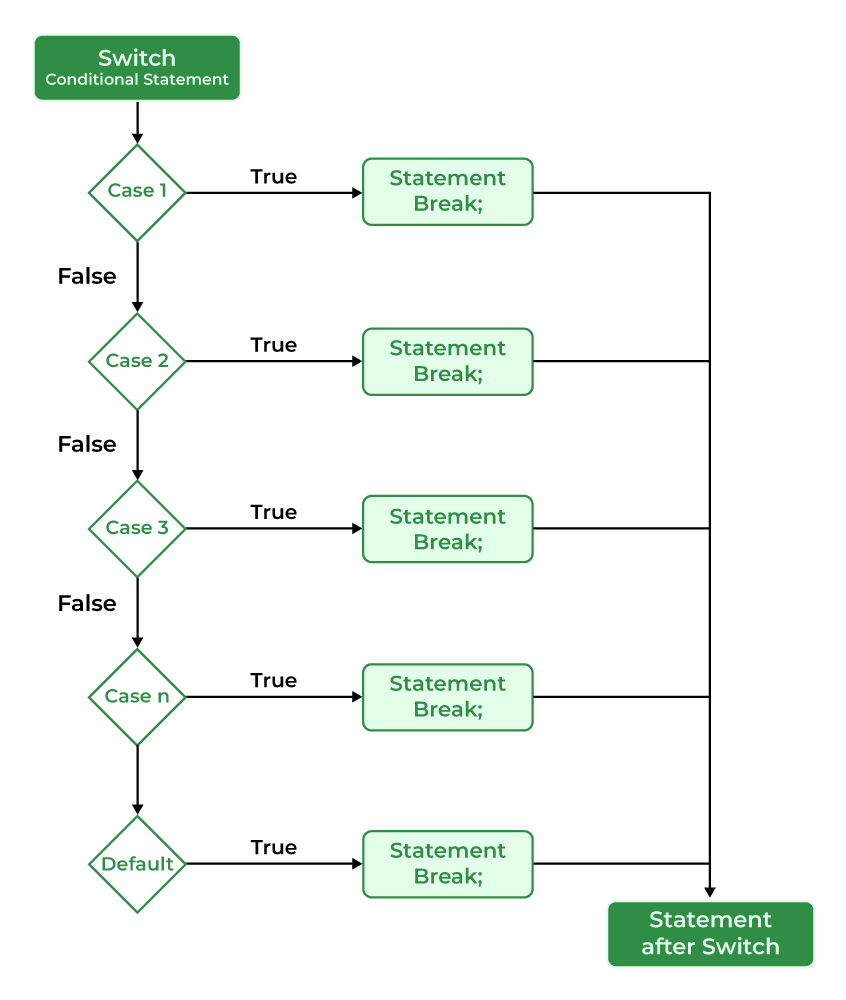
\includegraphics[width=0.7\textwidth]{figures/switch-case-in-c.png}
                        \caption{\label{fig:switch-case-in-c}Switch case in C}
                    \end{figure} 
        
            Here is an example to better understand:
            
            \begin{lstlisting}[style=mystyle_c, language=c, breaklines]
                        // C program to Demonstrate returning of day based numeric
                        // value
                        #include <stdio.h>
                         
                        int main()
                        {
                          // switch variable
                            int var = 1;
                         
                          // switch statement
                            switch (var) {
                                case 1:
                                    printf("Case 1 is Matched.");
                                    break;
                         
                                case 2:
                                    printf("Case 2 is Matched.");
                                    break;
                         
                                case 3:
                                    printf("Case 3 is Matched.");
                                    break;
                         
                                default:
                                    printf("Default case is Matched.");
                                    break;
                            }
                         
                            return 0;
                        }
                        \end{lstlisting}
        
        \subsection{Break and Continue}    
            You have already seen the break statement used in an earlier chapter of this tutorial. Interrupts the execution of a command (switch) or loop (for, while, do-while). The \textit{break} forces the output of the innermost loop.

            The \textit{continues} forces the execution of the next iteration of the loop



    \section{Functions} \label{sec:section_cl.5}

        Good C code is vastly superior to assembly code in terms of organization and readability, and this is due in large part to the use of functions.
            
        Functions are blocks of code that can be easily incorporated into other portions of code. Causing the processor to execute the instructions contained in the function is referred to as “calling” the function. A function can accept one or multiple inputs, and it can provide one output, called a return value.

        In a function declaration \autoref{fig:function-declaration-in-c}, we must provide the function name, its return type, and the number and type of its parameters. A function declaration tells the compiler that there is a function with the given name defined somewhere else in the program.
        The parameter name is not mandatory while declaring functions. We can also declare the function without using the name of the data variables.

        \begin{figure}[!ht]
                \centering
                \captionsetup{justification=centering,margin=0.05cm}
                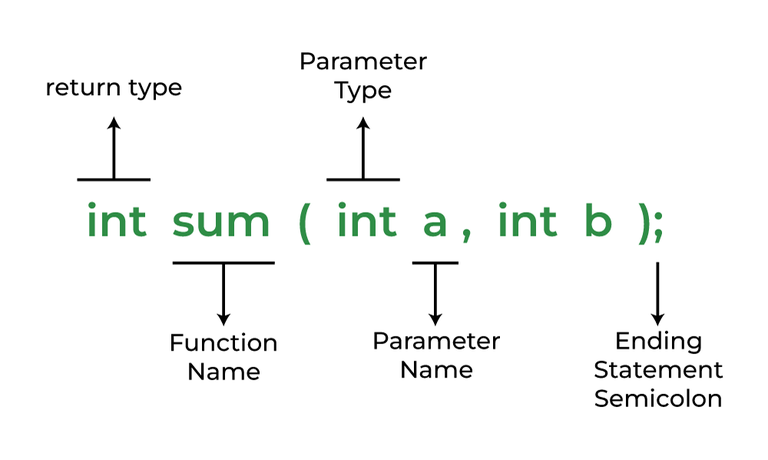
\includegraphics[width=0.7\textwidth]{figures/function-in-c.png}
                \caption{\label{fig:function-declaration-in-c}Function declaration}
        \end{figure}
        \vspace{0.5cm}
        In the below example \autoref{fig:working-of-function-in-c}, the first sum function is called and 10,30 are passed to the sum function. After the function call sum of a and b is returned and control is also returned back to the main function of the program.
        
        \begin{figure}[!ht]
                \centering
                \captionsetup{justification=centering,margin=0.05cm}
                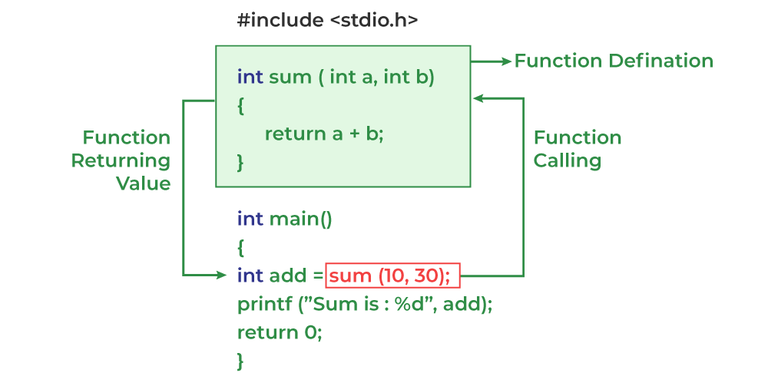
\includegraphics[width=0.7\textwidth]{figures/working-of-function-in-c.png}
                \caption{\label{fig:working-of-function-in-c}Working of Function}
        \end{figure}

        The data passed when the function is being invoked is known as the Actual parameters. In the below \autoref{fig:function-parameters-in-c}, 10 and 30 are known as actual parameters. Formal Parameters are the variable and the data type as mentioned in the function declaration. In the below program, a and b are known as formal parameters.

        \begin{figure}[!ht]
                \centering
                \captionsetup{justification=centering,margin=0.05cm}
                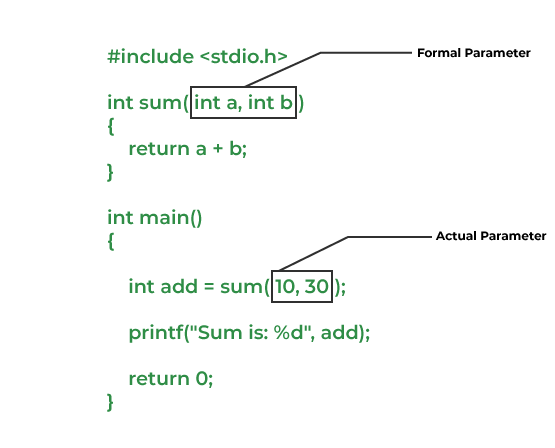
\includegraphics[width=0.7\textwidth]{figures/function-parameters-in-c.png}
                \caption{\label{fig:function-parameters-in-c}Passing parameters to functions}
        \end{figure}
        
        The use of functions does involve some overhead, so we have to be careful to not burden the processor with an excessive number of function calls, but in general the benefits of functions far outweigh the costs.
            
        Here is an example of a function that has three numerical inputs and uses these inputs to generate a true-or-false return value.
            
            \begin{lstlisting}[style=mystyle_c, language=c, breaklines]
                bit Is_In_Range(int input, int LowerBound, int UpperBound)
                {
                    if(input >= LowerBound && input <= UpperBound)
                        return TRUE;
                
                    else
                        return FALSE;
                }
            \end{lstlisting}